\documentclass[conference]{IEEEtran}
\IEEEoverridecommandlockouts

\usepackage{cite}
\usepackage{amsmath,amssymb,amsfonts}
\usepackage{algorithmic}
\usepackage{graphicx}
\usepackage{textcomp}
\usepackage{xcolor}
\usepackage{booktabs}
\usepackage{array}
\usepackage{multirow}
\usepackage{url}
\usepackage{hyperref}

\def\BibTeX{{\rm B\kern-.05em{\sc i\kern-.025em b}\kern-.08em
    T\kern-.1667em\lower.7ex\hbox{E}\kern-.125emX}}

\begin{document}

\title{When Agents Fail to Act: A Diagnostic Framework for Tool Invocation Reliability in Multi-Agent LLM Systems}

\author{
\IEEEauthorblockN{Donghao Huang\textsuperscript{1,2}, Gauri Malwe\textsuperscript{3},
 Zhaoxia Wang\textsuperscript{1}}
\IEEEauthorblockA{\textsuperscript{1}School of Computing and Information Systems, Singapore Management University, Singapore\\
\textsuperscript{2}Research and Development, Mastercard, Arlington, VA, USA\\
\textsuperscript{3}Research and Development, Mastercard, Pune, India}
\IEEEauthorblockA{
dh.huang.2023@smu.edu.sg, gauri.malwe@mastercard.com, zxwang@smu.edu.sg
}
}

\maketitle

\begin{abstract}
Multi-agent systems powered by large language models (LLMs) are transforming enterprise automation, yet systematic evaluation methodologies for assessing tool-use reliability remain underdeveloped. We introduce a comprehensive diagnostic framework that leverages big data analytics to evaluate procedural reliability in intelligent agent systems, addressing critical needs for SME-centric deployment in privacy-sensitive environments. Our approach features a 12-category error taxonomy capturing failure modes across tool initialization, parameter handling, execution, and result interpretation. Through systematic evaluation of 1,980 deterministic test instances spanning both open-weight models (Qwen2.5 series, Functionary) and proprietary alternatives (GPT-4, Claude 3.5/3.7) across diverse edge hardware configurations, we identify actionable reliability thresholds for production deployment. Our analysis reveals that procedural reliability---particularly tool initialization failures---constitutes the primary bottleneck for smaller models, while qwen2.5:32b achieves flawless performance matching GPT-4.1. The framework demonstrates that mid-sized models (qwen2.5:14b) offer practical accuracy-efficiency trade-offs on commodity hardware (96.6\% success rate, 7.3s latency), enabling cost-effective intelligent agent deployment for resource-constrained organizations. This work establishes foundational infrastructure for systematic reliability evaluation of tool-augmented multi-agent AI systems.
\end{abstract}

\begin{IEEEkeywords}
intelligent agents, multi-agent systems, large language models, tool-use reliability, error taxonomy
\end{IEEEkeywords}

\section{Introduction}
\label{sec:Introduction}

Multi-agent systems leveraging large language models (LLMs) for autonomous task execution represent a significant advancement in artificial intelligence~\cite{acharya2025agentic,hong2024metagpt}, yet their production deployment remains constrained by fundamental challenges in procedural reliability and systematic evaluation. While existing research demonstrates tool-augmented LLM capabilities across various domains~\cite{schick2023toolformer,shen2023hugginggpt,qin2023toolllm}, the field critically lacks comprehensive diagnostic frameworks for characterizing failure modes in multi-agent coordination scenarios where tools must be reliably invoked, parameterized, and validated.

Current evaluation approaches predominantly report aggregate task success rates~\cite{hendrycks2021measuring,zheng2024judging}, obscuring underlying failure causes and limiting opportunities for targeted improvements. Recent work by Kokane et al.~\cite{kokane2024spectool} demonstrates the value of granular error taxonomies for single-agent tool use, yet these frameworks remain insufficient for multi-agent contexts where failures cascade through coordination protocols. Chawla et al.~\cite{chawla2024agentic} identify tool use as a fundamental pillar of agentic AI, yet systematic reliability evaluation methodologies for multi-agent systems remain critically underdeveloped.

We address this gap by establishing a diagnostic framework that moves beyond aggregate metrics to provide actionable insights into specific failure patterns. Recognizing that organizations—particularly small and medium-sized enterprises (SMEs)—face diverse deployment constraints including hardware limitations, privacy requirements, and cost sensitivity~\cite{huang2025llms}, we establish a tiered framework characterizing reliability-cost trade-offs across model scales and hardware configurations. %While recent advances in quantization~\cite{frantar2023gptq,dettmers2023qlora} have made edge deployment increasingly feasible, the reliability implications of running quantized multi-agent systems on resource-constrained hardware remain poorly understood.

% We demonstrate our methodology through invoice reconciliation, a representative business automation task requiring multi-modal document processing, coordinated tool use, and database interactions.% This domain provides ideal evaluation conditions: clear ground truth, realistic multi-tool coordination complexity, and direct relevance to privacy-sensitive financial workflows.

Our contributions are:

\begin{enumerate}
    \item \textbf{Systematic Diagnostic Framework:} A novel 12-category error taxonomy spanning tool initialization, parameter handling, execution, and result interpretation, extending single-agent diagnostic capabilities~\cite{kokane2024spectool} to multi-agent coordination scenarios.
    
    \item \textbf{Reproducible Evaluation Infrastructure:} Standardized protocols comparing open-weight models (qwen2.5:3b through 72B, Functionary) against closed-source alternatives (GPT-4, Claude 3.5/3.7) across diverse edge hardware (NVIDIA RTX A6000, RTX 4090, Apple M3 Max) using 4-bit quantization for realistic deployment conditions.
    
    \item \textbf{Reliability Threshold Identification:} Quantitative analysis across 1,980 deterministic test instances identifying critical capacity thresholds—qwen2.5:32b achieves flawless reliability matching GPT-4.1, while qwen2.5:14b represents the minimum viable production configuration (96.6--97.4\% success).
    
    \item \textbf{Deployment Guidance and Open Resources:} Hardware-performance characterization demonstrating 8.2$\times$ latency variation across platforms, establishing practical deployment recommendations. All code, evaluation protocols, synthetic datasets, and analysis tools are publicly available to support reproducible research in multi-agent LLM reliability assessment.\footnote{\url{https://github.com/inflaton/df4tir}}
\end{enumerate}

% This diagnostic framework addresses a foundational gap in multi-agent LLM evaluation~\cite{acharya2025agentic,chen2021evaluating}, providing systematic tools for characterizing procedural reliability beyond aggregate success metrics. By establishing clear performance thresholds, identifying specific failure modes, and demonstrating open-weight parity with proprietary alternatives at sufficient scale, our work enables more rigorous assessment methodologies for tool-augmented agentic AI systems across domains.

\section{Related Work}
\label{sec:Related}

% CHANGE: Added paragraph discussing organizational approaches to multi-agent systems with the reviewer-requested citation
% Rationale: Reviewer requested citing Berrich et al. to enhance background; integrating it meaningfully into related work
% \noindent \textbf{Organizational Approaches to Multi-Agent Systems}
% Early work on multi-agent system organization provides foundational insights for understanding coordination challenges. Berrich et al.~\cite{berrich2012integration} demonstrated organizational approaches to multi-agent validation systems in e-learning contexts, highlighting how structured agent interactions can improve reliability in task execution. %While their work focused on educational applications, the principles of organizational structure and validation mechanisms inform our understanding of reliability requirements in tool-augmented agent systems.

\noindent\textbf{Multi-Agent LLM Systems and Coordination}
Berrich et al.~\cite{berrich2012integration} demonstrated that organizational approaches to multi-agent systems can improve task execution reliability.
Recent advances in LLM-based multi-agent systems have demonstrated significant potential for complex task automation. Acharya et al. provide a comprehensive survey of agentic AI systems, emphasizing the importance of systematic evaluation methodologies~\cite{acharya2025agentic}. Hong et al. introduced MetaGPT, demonstrating structured multi-agent coordination through role specialization~\cite{hong2024metagpt}, while Chawla et al. identify tool use as a fundamental pillar of agentic AI systems~\cite{chawla2024agentic}. %However, these works focus primarily on capability demonstration rather than systematic reliability assessment, highlighting the need for comprehensive diagnostic frameworks.

\noindent \textbf{Tool-Use Evaluation and Error Analysis}
Understanding failure modes in tool-augmented LLMs represents an emerging but critical research area. Kokane et al. argue for moving beyond simple success rates to systematic error characterization, introducing SpecTool with seven error categories for single-agent tool-use evaluation~\cite{kokane2024spectool}. Their work demonstrates that even state-of-the-art models exhibit systematic tool-use failures, but focuses on single-agent scenarios without addressing the coordination challenges inherent in multi-agent systems.
% Recent work by ~\cite{kokane2024spectool} and similar studies reveal the importance of granular error analysis, yet existing taxonomies remain insufficient for multi-agent contexts where tool failures can cascade through agent coordination protocols. %Our work extends this foundation by developing systematic diagnostic methodologies specifically designed for multi-agent tool-use scenarios.

\noindent \textbf{Edge Deployment and Model Optimization}
The deployment of LLMs on resource-constrained hardware has garnered significant attention due to privacy and cost considerations. 
Frantar et al. and Dettmers et al. demonstrate that 4-bit quantization can dramatically reduce memory requirements while maintaining performance for single-model inference~\cite{frantar2023gptq,dettmers2023qlora}.
% Qu et al. and Dettmers et al. demonstrate that 4-bit quantization can dramatically reduce memory requirements while maintaining performance for single-model inference. 
Huang and Wang extend this work to multi-model scenarios, showing that medium-sized models (7B–32B parameters) achieve optimal performance-efficiency trade-offs on edge hardware~\cite{huang2025llms}.
% However, existing edge deployment research focuses primarily on single-model inference rather than the complex orchestration requirements of multi-agent systems. %Our work addresses this gap by systematically evaluating multi-agent coordination reliability under realistic hardware constraints.

\noindent \textbf{LLM Reliability and Failure Analysis.}
Despite substantial research on LLM performance evaluation~\cite{hendrycks2021measuring,zheng2024judging,chen2021evaluating}, systematic diagnostic frameworks for multi-agent reliability remain critically underdeveloped. Traditional evaluation methodologies prioritize aggregate success metrics—such as task completion rates or accuracy scores—that obscure the underlying causes of system failures~\cite{kokane2024spectool}. While recent work has begun examining single-agent tool-use errors~\cite{kokane2024spectool} and benchmarking capabilities on isolated tasks~\cite{qin2023toolllm,schick2023toolformer}, these approaches do not address the coordination challenges and cascading failure modes inherent in multi-agent architectures. %Our diagnostic framework fills this gap by providing fine-grained, multi-dimensional failure characterization across agent interactions, tool invocations, and workflow orchestration. This granular analysis enables targeted system improvements—such as prompt refinement, architectural modifications, and validation layer design—and supports evidence-based deployment decisions tailored to organizational constraints.

\subsection{Diagnostic Framework Overview}

Our diagnostic framework provides systematic methodology for evaluating procedural reliability in multi-agent LLM systems through three core components: (1) structured error taxonomy for comprehensive failure characterization, (2) standardized evaluation protocols for reproducible assessment, and (3) hardware-performance characterization for deployment guidance.

The framework is designed for broad applicability across multi-agent scenarios while maintaining diagnostic precision through domain-specific instantiation. We demonstrate this approach using invoice reconciliation as a representative case study of structured business automation requiring multi-modal processing and coordinated tool use.

\subsection{Multi-Agent System Architecture}

\begin{figure}[t]
    \centering
    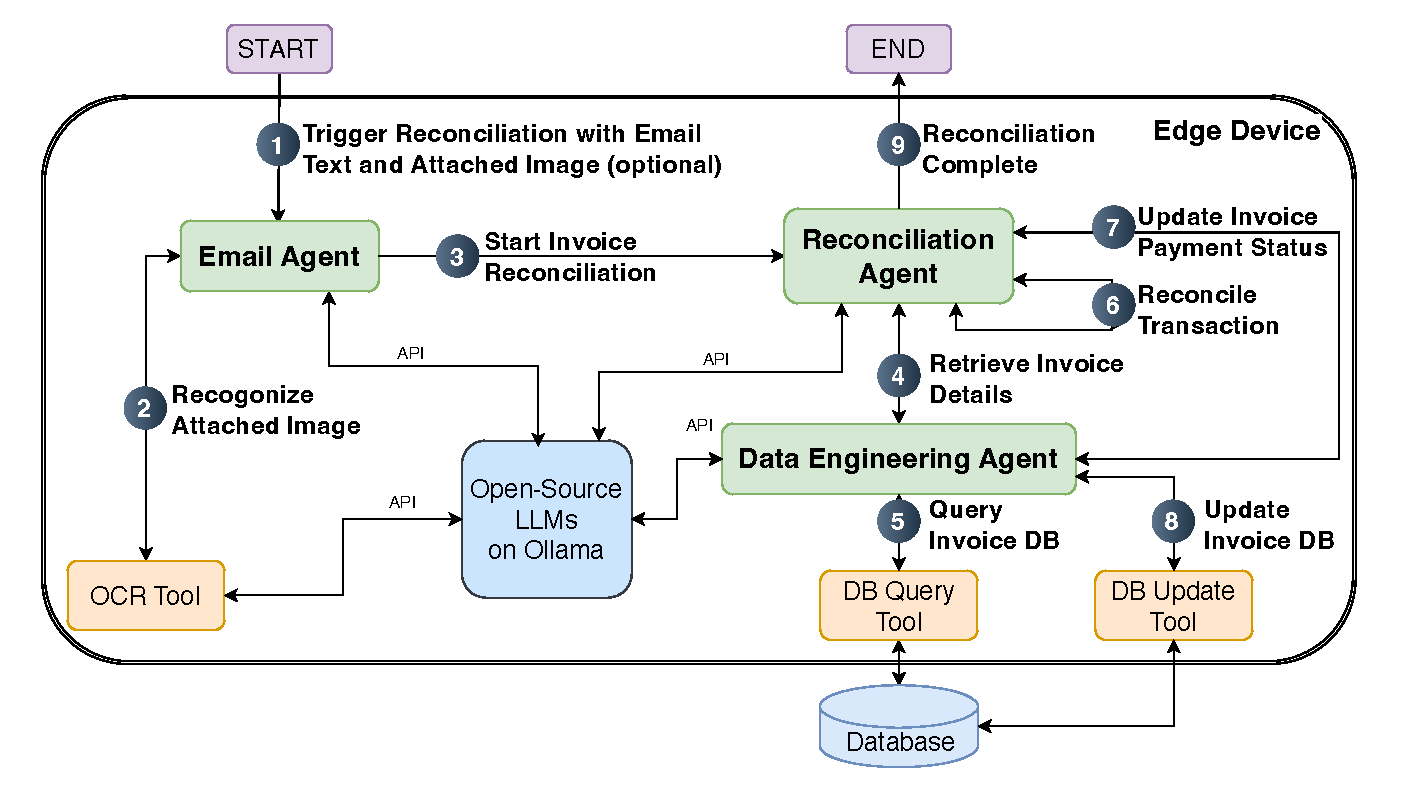
\includegraphics[width=\linewidth]{images/Multi_Agents_v1.drawio.pdf}
    \caption{Multi-agent system architecture demonstrating our diagnostic framework. Three specialized agents coordinate through LangGraph orchestration: Email Agent (input processing and OCR), Data Engineering Agent (database operations), and Reconciliation Agent (workflow coordination). Our error taxonomy systematically captures failures across all tool interactions and agent coordination points.}
    \label{fig:architecture}
    \vspace{-1.5em}
\end{figure}

Building upon our previous work on edge-deployed LLM systems for invoice reconciliation~\cite{huang2025scalable}, we implement a modular three-agent architecture orchestrated through LangGraph (Figure~\ref{fig:architecture}). While the prior work demonstrated practical feasibility and resource efficiency of edge deployment, the current work extends this foundation by introducing comprehensive diagnostic capabilities to systematically characterize procedural reliability across model scales and hardware configurations.

The architecture comprises three specialized agents, each enhanced with detailed instrumentation for failure diagnosis:

\begin{itemize}
\item \textbf{Email Agent}: Processes input documents and manages OCR tool invocation for multi-modal content analysis. Enhanced with logging mechanisms to capture OCR initialization failures, parameter mismatches, execution errors, and result interpretation issues.

\item \textbf{Data Engineering Agent}: Executes structured database operations through \texttt{DB Query Tool} and \texttt{DB Update Tool} with validation and error handling. Instrumented to identify query construction failures, schema validation errors, and update operation anomalies.

\item \textbf{Reconciliation Agent}: Coordinates workflow execution, processes agent outputs, and makes final reconciliation decisions. Monitors inter-agent communication failures and coordination breakdowns.
\end{itemize}

% While our previous system~\cite{huang2025scalable} focused on achieving high task success rates (99.9\% with qwen2.5:32b) and practical resource efficiency, it provided limited visibility into \emph{why} and \emph{how} failures occurred. The current work addresses this gap by:

% \begin{enumerate}
%     \item \textbf{Comprehensive Error Instrumentation}: Every tool invocation is logged with detailed execution traces, enabling post-hoc failure analysis through our 12-category taxonomy.
    
%     \item \textbf{Expanded Model Evaluation}: Beyond the original model set (qwen2.5:7b/32b/72b, functionary-small/medium), we evaluate additional model scales (qwen2.5:3b, 14B) and proprietary alternatives (GPT-4 variants, Claude 3.5/3.7) to establish reliability thresholds across the performance spectrum.
    
%     \item \textbf{Systematic Hardware Characterization}: Extended evaluation across three hardware platforms (RTX A6000, RTX 4090, M3 Max) with identical experimental protocols, providing reproducible hardware-performance relationships absent in prior work.
    
%     \item \textbf{Deterministic Evaluation Protocol}: Standardized evaluation with fixed prompts, no sampling variance, and complete logging of all 1,980 task instances, enabling stable diagnostic metrics and systematic failure pattern identification.
% \end{enumerate}

This architecture enables systematic evaluation of tool-use reliability across multiple coordination scenarios while maintaining clear diagnostic boundaries for failure attribution. The modular design supports comprehensive model comparison by isolating LLM performance from orchestration framework effects, allowing us to identify whether failures stem from model capacity limitations, prompt design issues, or architectural constraints.

% Importantly, the diagnostic framework is model-agnostic and can be applied to any LLM backend, making our findings generalizable beyond the specific models evaluated. The error taxonomy and evaluation protocols provide standardized infrastructure for future research in multi-agent reliability assessment.

\subsection{Error Taxonomy for Multi-Agent Tool Use}

Our diagnostic framework centers on a systematic error taxonomy that provides fine-grained characterization of tool-use failures in multi-agent systems. The taxonomy systematically combines four error types with three tool categories, yielding twelve distinct failure modes.

\textbf{Error Type Categories:}
\begin{itemize}
    \item \textbf{Not Initialized:} Agent fails to properly invoke tool due to malformed calls, incorrect tool names, or invalid parameter structures.
    \item \textbf{Args Mismatch:} Tool invocation succeeds but contains incorrect or invalid arguments leading to tool-specific failures.
    \item \textbf{Error:} Tool executes with valid parameters but returns runtime errors or exceptions.
    \item \textbf{Result Mismatch:} Tool execution succeeds but produces outputs that cause downstream task failure.
\end{itemize}

\textbf{Tool Categories:} OCR processing, database query operations, and database update operations, representing common primitives in structured business automation for invoice reconciliation.

\textbf{Complete Taxonomy.} The cross-product of four error types and three tool categories produces the following 12 diagnostic categories used throughout our evaluation:

\begin{enumerate}
    \item \texttt{OCR\_TOOL\_NOT\_INITIALIZED}: Failure to invoke OCR tool
    \item \texttt{OCR\_TOOL\_ARGS\_MISMATCH}: OCR tool called with invalid arguments
    \item \texttt{OCR\_TOOL\_ERROR}: OCR tool execution returns runtime errors
    \item \texttt{OCR\_TOOL\_RESULT\_MISMATCH}: OCR output causes downstream failures
    \item \texttt{DB\_QUERY\_TOOL\_NOT\_INITIALIZED}: Failure to invoke database query tool
    \item \texttt{DB\_QUERY\_TOOL\_ARGS\_MISMATCH}: Query tool called with invalid arguments
    \item \texttt{DB\_QUERY\_TOOL\_ERROR}: Query execution returns runtime errors
    \item \texttt{DB\_QUERY\_TOOL\_RESULT\_MISMATCH}: Query results cause downstream failures
    \item \texttt{DB\_UPDATE\_TOOL\_NOT\_INITIALIZED}: Failure to invoke database update tool
    \item \texttt{DB\_UPDATE\_TOOL\_ARGS\_MISMATCH}: Update tool called with invalid arguments
    \item \texttt{DB\_UPDATE\_TOOL\_ERROR}: Update execution returns runtime errors
    \item \texttt{DB\_UPDATE\_TOOL\_RESULT\_MISMATCH}: Update results cause downstream failures
\end{enumerate}

% Each error instance is logged with complete execution context including agent state, tool invocation parameters, and orchestration trace, enabling post-hoc failure analysis. This taxonomy enables systematic identification of reliability bottlenecks and provides actionable diagnostic information for system improvement. Unlike aggregate success metrics, our framework reveals specific failure patterns that enable targeted interventions in model selection, prompt engineering, and system architecture.

\subsection{Evaluation Dataset}

We establish standardized evaluation protocols using a carefully constructed synthetic dataset mirroring real-world invoice reconciliation scenarios. The dataset comprises 1,980 test instances balanced between vision-enabled (990) and text-only (990) tasks.

Our evaluation focuses on positive reconciliation cases—scenarios where invoices are fully paid and records should match across email, receipt, and database entries. This controlled approach enables systematic baseline assessment of procedural reliability without confounding factors from exception handling, providing essential diagnostic infrastructure for the research community.

\subsection{LLM Integration}

\textbf{Model Selection.} To establish comprehensive reliability benchmarks across the performance spectrum, we evaluate two categories of LLMs:

\begin{itemize}
\item \textbf{Closed-Source Models:} OpenAI's GPT-4 series (gpt-4o, gpt-4o-mini, gpt-4.1-nano, gpt-4.1-mini, gpt-4.1) and Anthropic's Claude models (3.5 Sonnet, 3.7 Sonnet) serve as reference baselines representing state-of-the-art proprietary systems.

\item \textbf{Open-Weight Models:} The Qwen2.5 series (3B, 7B, 14B, 32B, 72B) and Functionary V3.1 (8B, 70B) offer systematic coverage across model scales, with local deployment ensuring data sovereignty. For models lacking native vision capabilities, Llama3.2-Vision-11B performs OCR tasks, enabling fair comparisons with multimodal closed-source counterparts.
\end{itemize}

\textbf{Deployment Configuration.} All open-weight models were executed locally using Ollama\footnote{\url{https://ollama.com/}} v0.6.8 with 4-bit quantization (Q4\_K\_M format) to simulate realistic edge deployment constraints while maintaining acceptable inference quality. Closed-source models were accessed via their respective APIs, with all timing measurements including full round-trip network latency to ensure fair performance comparison against local inference.

\textbf{Hardware Infrastructure.} To evaluate deployment trade-offs across diverse environments, all open-weight models are tested on three representative edge platforms spanning a range of cost-performance profiles:

\begin{itemize}
\item \textbf{NVIDIA RTX A6000 Ada GPU:} A high-end workstation GPU (48GB VRAM, Ubuntu 24.04, \textasciitilde\$10K), referred to as \textit{RTX A6000}.

\item \textbf{NVIDIA GeForce RTX 4090 Laptop GPU:} A mobile workstation setup (16GB VRAM, Ubuntu 24.04 via WSL, \textasciitilde\$5K), referred to as \textit{RTX 4090}.

\item \textbf{Apple M3 Max:} A consumer-grade ARM platform (96GB unified memory, macOS 15.4.1, \textasciitilde\$4K), referred to as \textit{M3 Max}.
\end{itemize}

% This multi-platform evaluation characterizes hardware-performance relationships essential for evidence-based deployment planning, enabling organizations to select configurations aligned with their reliability requirements, budget constraints, and operational context.

\subsection{Evaluation Metrics and Protocol}

Our evaluation employs four complementary metrics that together provide comprehensive reliability assessment:

\begin{itemize}
\item \textbf{Success Rate (SR):} The percentage of tasks completed without any tool-use errors, serving as the primary measure of end-to-end system reliability. A task is marked successful only when all required operations—OCR extraction (when applicable), database queries, and status updates—execute correctly without triggering any error in our 12-category taxonomy.

\item \textbf{Execution Time:} End-to-end task completion latency (seconds) measured from initial input processing through final database update, including all agent coordination overhead, tool invocation delays, and inter-agent communication. For API-based closed-source models, measurements capture complete network round-trip time to ensure fair comparison against local inference.

\item \textbf{Process Steps:} The total number of agent actions and tool invocations required to complete each task, providing insight into workflow efficiency and planning quality. Excessive steps indicate suboptimal planning, potential decision loops, or redundant operations—behavioral patterns particularly prevalent in smaller models struggling with multi-agent coordination.

\item \textbf{OCR F1 Score:} For vision-based tasks (990 instances with receipt images), we compute BERT F1 score~\cite{zhang2020bertscore} to quantify semantic similarity between OCR-extracted text and ground truth transcriptions. This metric isolates text recognition quality from downstream reconciliation performance, enabling independent assessment of vision processing capabilities.
\end{itemize}

\textbf{Evaluation Protocol.} All experiments employ deterministic execution (temperature=0, fixed prompts) across 1,980 test instances evenly split between vision-based (990) and text-only (990) workflows. This deterministic approach eliminates sampling variance, ensuring reproducible diagnostic assessment. Each model configuration executes exactly once per test instance, with complete execution traces logged for comprehensive error analysis through our 12-category taxonomy.

% For multi-platform evaluations (RTX A6000, RTX 4090, M3 Max), identical prompts, quantization settings (Q4\_K\_M), and orchestration parameters are maintained across all open-weight models. This standardization ensures that observed performance variations reflect genuine hardware-model interactions rather than configuration artifacts. Success rates, execution times, and process steps are aggregated across all 1,980 instances; OCR F1 scores are computed exclusively for the 990 vision-enabled tasks.

The combination of aggregate system metrics (success rate, execution time) with diagnostic indicators (process steps, OCR quality) and fine-grained error taxonomy enables comprehensive reliability characterization essential for evidence-based deployment decisions in resource-constrained environments.

\textbf{Qualitative Failure Analysis.}
To complement our quantitative error taxonomy, we conduct systematic qualitative analysis of failure patterns. This analysis focuses specifically on initialization failures—the dominant error type revealed by our taxonomy—to identify the underlying reasoning deficiencies that lead to systematic tool-use breakdowns.

% This qualitative characterization provides actionable insights for targeted interventions, including prompt engineering refinements, model training improvements, and system architecture enhancements to mitigate specific failure modes.

%%%%%%%%%%%%%%%%%%%%%%%%%%%%%%%%%%%%%%%%%%%%%%%%%%%%%%%%%%%%%%%%%%%%%%%%
% RESULTS AND ANALYSIS SECTION
%%%%%%%%%%%%%%%%%%%%%%%%%%%%%%%%%%%%%%%%%%%%%%%%%%%%%%%%%%%%%%%%%%%%%%%%

\section{Results and Analysis}
\label{sec:Results}

% Our diagnostic framework reveals systematic patterns in multi-agent tool-use reliability that provide actionable insights for deployment and model selection. We present comprehensive analysis across performance metrics, error characterization, and hardware trade-offs.

%%%%%%%%%%%%%%%%%%%%%%%%%%%%%%%%%%%%%%%%%%%%%%%%%%%%%%%%%%%%%%%%%%%%%%%%
\subsection{Performance and Reliability Trade-offs}
%%%%%%%%%%%%%%%%%%%%%%%%%%%%%%%%%%%%%%%%%%%%%%%%%%%%%%%%%%%%%%%%%%%%%%%%

Table~\ref{tab:accuracy_overall} summarizes overall performance metrics for all evaluated LLM configurations and is visualized in Figure~\ref{fig:perf_metrics}. Detailed results for vision-based and text-only workflows are presented in Tables~\ref{tab:accuracy_vision} and~\ref{tab:accuracy_nonvision}, respectively. %Success rate (SR) reflects the percentage of tasks completed without errors, and execution time is reported as mean~$\pm$~standard deviation. For open-weight models tested across multiple platforms, hardware environment notably impacts both reliability and latency.

%%%%%%%%%%%%%%%%%%%%%%%%%%%%%%%%%%%%%%%%%%%%%%%%%%%%%%%%%%%%%%%%%%%%%%%%
% TABLES (same as before, but with improved captions)
%%%%%%%%%%%%%%%%%%%%%%%%%%%%%%%%%%%%%%%%%%%%%%%%%%%%%%%%%%%%%%%%%%%%%%%%

\begin{table}[htbp]
\centering
\caption{Overall invoice reconciliation performance across LLM configurations.}
\label{tab:accuracy_overall}
\resizebox{\columnwidth}{!}{%
\begin{tabular}{llccc}
\toprule
\textbf{Model} & \textbf{Platform} & \textbf{SR (\%)} & \textbf{Time (s)} & \textbf{Steps} \\
\midrule
\multicolumn{5}{l}{\textit{Closed-source models}} \\
gpt-4o-mini & OpenAI & 99.3 & \textbf{7.6 ± 1.6} & 8.6 ± 1.2 \\
gpt-4o & OpenAI & 98.8 & 12.4 ± 13.2 & 8.5 ± 0.6 \\
gpt-4.1-nano & OpenAI & 85.7 & 8.6 ± 12.3 & 18.5 ± 18.6 \\
gpt-4.1-mini & OpenAI & 99.5 & 8.6 ± 2.7 & 9.6 ± 1.9 \\
gpt-4.1 & OpenAI & \textbf{100.0} & 8.3 ± 7.7 & 9.9 ± 9.7 \\
claude-3-5-sonnet & Anthropic & 97.8 & 18.7 ± 6.3 & 8.5 ± 0.5 \\
claude-3-7-sonnet & Anthropic & 99.3 & 16.8 ± 12.3 & 8.5 ± 0.7 \\
\midrule
\multicolumn{5}{l}{\textit{Open-weight models}} \\
\multirow{3}{*}{qwen2.5:3b} & RTX 4090 & 13.1 & 11.0 ± 31.1 & 17.2 ± 12.5 \\
 & RTX A6000 & 13.9 & 8.1 ± 19.0 & 18.8 ± 14.7 \\
 & M3 Max & 14.9 & 45.9 ± 95.3 & 16.4 ± 11.9 \\
\multirow{3}{*}{qwen2.5:7b} & RTX 4090 & 49.3 & 12.6 ± 14.7 & 16.9 ± 20.3 \\
 & RTX A6000 & 57.3 & 9.9 ± 10.2 & 20.7 ± 22.0 \\
 & M3 Max & 58.5 & 85.9 ± 95.9 & 20.7 ± 21.3 \\
\multirow{3}{*}{qwen2.5:14b} & RTX 4090 & 97.4 & 12.5 ± 11.3 & 8.6 ± 2.1 \\
 & RTX A6000 & 96.6 & \textbf{7.3 ± 8.0} & 8.6 ± 2.2 \\
 & M3 Max & 97.0 & 60.0 ± 20.5 & 8.6 ± 1.7 \\
qwen2.5:32b & RTX A6000 & \textbf{100.0} & 13.9 ± 16.9 & 8.5 ± 0.5 \\
qwen2.5:72b & RTX A6000 & 95.1 & 39.3 ± 24.8 & 8.7 ± 4.2 \\
functionary-small & RTX A6000 & 7.5 & 4.0 ± 21.6 & 5.6 ± 3.7 \\
functionary-medium & RTX A6000 & 53.2 & 30.8 ± 242.6 & 7.8 ± 2.8 \\
\bottomrule
\end{tabular}%
}
\vspace{0.1cm}

\footnotesize{\textbf{Note:} 
%Open-weight models (Qwen2.5 and functionary) were run locally with 4-bit quantization (Q4\_K\_M). OpenAI and Anthropic models were accessed via their cloud APIs. 
SR = Success Rate. Execution times include full network latency for API-based models. All metrics based on 1,980 test instances
% (990 vision, 990 non-vision)
.}
\end{table}

\begin{table*}[htbp]
\centering
\caption{Vision task performance including OCR BERT F1 scores.}
\label{tab:accuracy_vision}
\resizebox{.75\textwidth}{!}{%
\begin{tabular}{lllcccc}
\toprule
\textbf{Type} & \textbf{Model} & \textbf{Platform} & \textbf{SR (\%)} & \textbf{Time (s)} & \textbf{Steps} & \textbf{OCR F1} \\
\midrule
Closed & gpt-4o-mini & OpenAI & 99.5 & 7.8 ± 1.5 & 9.3 ± 1.2 & 0.949 ± 0.008 \\
Closed & gpt-4o & OpenAI & 98.8 & 14.2 ± 16.1 & 9.0 ± 0.5 & 0.916 ± 0.029 \\
Closed & gpt-4.1-nano & OpenAI & 90.9 & \textbf{7.4 ± 6.1} & 15.9 ± 8.3 & \textbf{0.950 ± 0.031} \\
Closed & gpt-4.1-mini & OpenAI & 99.1 & 10.5 ± 2.5 & 11.1 ± 1.4 & 0.916 ± 0.008 \\
Closed & gpt-4.1 & OpenAI & \textbf{100.0} & 10.3 ± 10.5 & 11.9 ± 13.5 & 0.934 ± 0.030 \\
Closed & claude-3-5-sonnet & Anthropic & 96.5 & 21.2 ± 7.4 & 9.0 ± 0.4 & \textbf{0.950 ± 0.061} \\
Closed & claude-3-7-sonnet & Anthropic & 98.7 & 18.1 ± 8.5 & 9.0 ± 0.7 & 0.936 ± 0.052 \\
\midrule
\multirow{3}{*}{Open} & \multirow{3}{*}{qwen2.5:3b} & RTX 4090 & 8.4 & 9.6 ± 42.1 & 12.7 ± 7.1 & 0.993 ± 0.035 \\
 &  & RTX A6000 & 7.2 & \textbf{6.4 ± 19.9} & 13.0 ± 8.8 & 0.994 ± 0.034 \\
 &  & M3 Max & 9.5 & 55.7 ± 80.0 & 12.9 ± 7.8 & 0.992 ± 0.035 \\
\multirow{3}{*}{Open} & \multirow{3}{*}{qwen2.5:7b} & RTX 4090 & 25.1 & 9.2 ± 14.8 & 12.9 ± 19.9 & 0.386 ± 0.485 \\
 &  & RTX A6000 & 42.1 & 9.2 ± 11.4 & 18.5 ± 22.1 & 0.624 ± 0.481 \\
 &  & M3 Max & 46.9 & 98.8 ± 104.3 & 19.9 ± 21.8 & 0.632 ± 0.474 \\
\multirow{3}{*}{Open} & \multirow{3}{*}{qwen2.5:14b} & RTX 4090 & 96.0 & 14.8 ± 15.2 & 9.1 ± 1.9 & 0.994 ± 0.014 \\
 &  & RTX A6000 & 94.6 & 7.8 ± 11.0 & 9.1 ± 2.5 & 0.994 ± 0.014 \\
 &  & M3 Max & 95.2 & 75.2 ± 16.3 & 9.1 ± 2.1 & 0.994 ± 0.014 \\
Open & qwen2.5:32b & RTX A6000 & \textbf{100.0} & 14.3 ± 23.9 & 9.0 ± 0.0 & \textbf{0.995 ± 0.013} \\
Open & qwen2.5:72b & RTX A6000 & 96.0 & 32.4 ± 16.1 & 9.7 ± 5.6 & 0.994 ± 0.013 \\
Open & functionary-small & RTX A6000 & 7.9 & 4.5 ± 8.5 & 6.1 ± 4.2 & 0.862 ± 0.340 \\
Open & functionary-medium & RTX A6000 & 39.8 & 28.9 ± 195.1 & 7.6 ± 3.1 & 0.995 ± 0.013 \\
\bottomrule
\end{tabular}%
}
\vspace{0.1cm}

\footnotesize{\textbf{Note:} 
%Open-weight models (Qwen2.5 and functionary) were run locally with 4-bit quantization (Q4\_K\_M). OpenAI and Anthropic models were accessed via their cloud APIs. 
SR = Success Rate. OCR F1 = OCR BERT F1 score measuring text recognition quality using semantic similarity. Type indicates Closed (cloud API) or Open (local inference). Open-weight models use Llama3.2-Vision-11B for OCR tasks. All results based on 990 vision tasks with attached receipt images.}
\end{table*}

\begin{table}[htbp]
\centering
\caption{Non-vision task performance.}
\label{tab:accuracy_nonvision}
\resizebox{\columnwidth}{!}{%
\begin{tabular}{llccc}
\toprule
\textbf{Model} & \textbf{Platform} & \textbf{SR (\%)} & \textbf{Time (s)} & \textbf{Steps} \\
\midrule
\multicolumn{5}{l}{\textit{Closed-source models}} \\
gpt-4o-mini & OpenAI & 99.1 & 7.3 ± 1.5 & 8.0 ± 0.5 \\
gpt-4o & OpenAI & 98.9 & 10.7 ± 9.1 & 8.0 ± 0.2 \\
gpt-4.1-nano & OpenAI & 80.4 & 9.8 ± 16.1 & 21.1 ± 24.6 \\
gpt-4.1-mini & OpenAI & \textbf{100.0} & 6.8 ± 1.4 & 8.0 ± 0.0 \\
gpt-4.1 & OpenAI & \textbf{100.0} & \textbf{6.4 ± 1.3} & 8.0 ± 0.0 \\
claude-3-5-sonnet & Anthropic & 99.1 & 16.1 ± 3.5 & 8.0 ± 0.0 \\
claude-3-7-sonnet & Anthropic & 99.9 & 15.4 ± 15.0 & 8.1 ± 0.4 \\
\midrule
\multicolumn{5}{l}{\textit{Open-weight models}} \\
\multirow{3}{*}{qwen2.5:3b} & RTX 4090 & 17.9 & 12.3 ± 12.5 & 21.8 ± 14.9 \\
 & RTX A6000 & 20.7 & 9.8 ± 17.9 & 24.5 ± 17.1 \\
 & M3 Max & 20.3 & 36.0 ± 107.7 & 20.0 ± 14.0 \\
\multirow{3}{*}{qwen2.5:7b} & RTX 4090 & 73.6 & 15.9 ± 13.8 & 20.8 ± 19.9 \\
 & RTX A6000 & 72.4 & 10.6 ± 8.9 & 22.9 ± 21.6 \\
 & M3 Max & 70.2 & 72.9 ± 84.9 & 21.5 ± 20.8 \\
\multirow{3}{*}{qwen2.5:14b} & RTX 4090 & 98.8 & 10.2 ± 3.5 & 8.1 ± 2.2 \\
 & RTX A6000 & 98.6 & \textbf{6.8 ± 2.3} & 8.1 ± 1.8 \\
 & M3 Max & 98.9 & 44.9 ± 10.9 & 8.0 ± 0.6 \\
qwen2.5:32b & RTX A6000 & \textbf{100.0} & 13.4 ± 1.4 & 8.0 ± 0.0 \\
qwen2.5:72b & RTX A6000 & 94.2 & 46.1 ± 29.7 & 7.8 ± 1.7 \\
functionary-small & RTX A6000 & 7.1 & 3.6 ± 29.4 & 5.1 ± 2.9 \\
functionary-medium & RTX A6000 & 66.6 & 32.7 ± 282.3 & 8.1 ± 2.5 \\
\bottomrule
\end{tabular}%
}
\vspace{0.1cm}

\footnotesize{\textbf{Note:} Open-weight models (Qwen2.5 and functionary) were run locally with 4-bit quantization (Q4\_K\_M). OpenAI and Anthropic models were accessed via their cloud APIs. SR = Success Rate. Non-vision tasks involve text-based workflows only, without image processing or OCR requirements. Payment confirmation details are provided directly in email text. All metrics based on 990 non-vision test instances.}
\end{table}

%%%%%%%%%%%%%%%%%%%%%%%%%%%%%%%%%%%%%%%%%%%%%%%%%%%%%%%%%%%%%%%%%%%%%%%%

\begin{figure*}[ht]
    \centering
    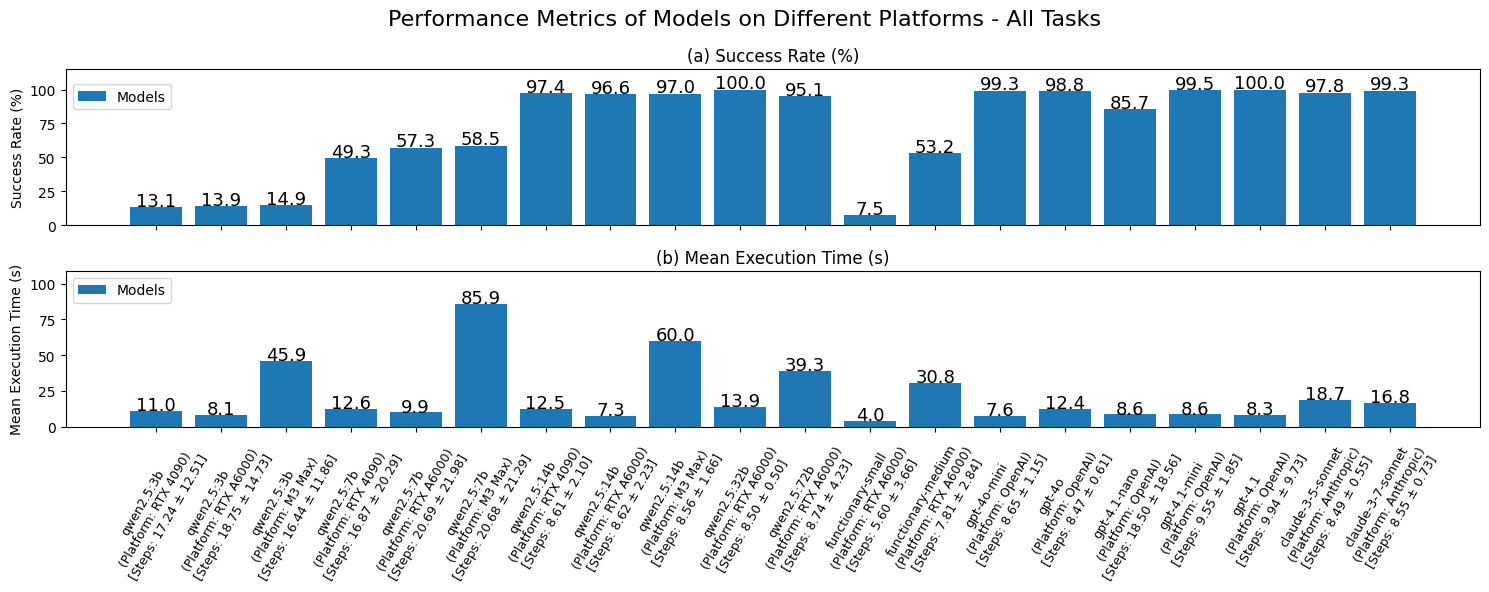
\includegraphics[width=.9\textwidth]{images/perf_metrics.png}
    \caption{Systematic performance analysis across models and hardware. \textbf{(a)} Task success rates reveal clear reliability thresholds at 14B and 32B parameters. \textbf{(b)} Execution times demonstrate significant hardware impact, with 8$\times$ variation between platforms for identical models.}
    \label{fig:perf_metrics}
    \vspace{-1em}
\end{figure*}

\paragraph{Reliability Thresholds.}
Our analysis reveals clear performance thresholds informing deployment decisions:

\begin{itemize}
    \item \textbf{Flawless performance:} qwen2.5:32b achieves perfect 100\% success matching GPT-4.1, demonstrating that open-weight models can achieve closed-source reliability at sufficient scale.
    
    \item \textbf{Production threshold:} qwen2.5:14b maintains 96.6--97.4\% success across all hardware platforms, establishing a practical reliability threshold for cost-sensitive deployments.
    
    \item \textbf{Diminishing returns:} qwen2.5:72b exhibits slightly lower success (95.1\%) than its 32B counterpart, suggesting task-specific capacity limits beyond which additional parameters provide minimal benefit.

    \item \textbf{Fundamental limits:} Smaller models exhibit significant performance degradation—qwen2.5:7b achieves 49.3--58.5\%, while qwen2.5:3b drops to 13.1--14.9\%—highlighting fundamental capacity constraints in complex multi-agent coordination.
\end{itemize}

\paragraph{Hardware Impact on Deployment Viability.}
Platform selection critically affects both latency and reliability:

\begin{itemize}
    \item \textbf{Hardware optimization:} qwen2.5:14b executes in 7.3~seconds on RTX A6000 versus 60.0~seconds on M3 Max—an 8.2$\times$ difference highlighting optimized hardware importance.
    
    \item \textbf{Planning efficiency matters:} Hardware alone is insufficient. qwen2.5:7b on M3 Max averages 85.9~seconds despite smaller size, requiring 20.7~steps per task versus 8.6~steps for the larger 14B model.

    \item \textbf{Pathological behavior:} Execution logs show that qwen2.5:7b often enters cyclical decision loops, occasionally exceeding LangGraph's recursion limit (25 steps) and triggering forced termination. This suggests that planning efficiency improves with model capacity.
\end{itemize}

\paragraph{Tiered Deployment Recommendations.}
Our framework supports evidence-based deployment across organizational constraints:

\begin{enumerate}
    \item \textbf{Maximum Reliability:} qwen2.5:32b on RTX A6000 (\$10K) achieves flawless performance comparable to GPT-4.1 while maintaining data sovereignty.
    
    \item \textbf{Balanced Performance:} qwen2.5:14b on RTX 4090 (\$5K) provides 96.6\% reliability—the optimal choice for most SME deployments.
    
    \item \textbf{Budget-Constrained:} Models below 14B require additional validation layers, automated retry mechanisms, and acceptance of higher failure rates for production use.
\end{enumerate}

\paragraph{Vision vs. Non-Vision Task Performance.}
Comparing Tables~\ref{tab:accuracy_vision} and~\ref{tab:accuracy_nonvision}, most models perform similarly across both modalities, with only minor differences. For vision tasks, OCR BERT F1 scores indicate that top-performing models achieve excellent text recognition quality (scores exceeding 0.99). The notable exception is qwen2.5:7b, which demonstrates inconsistent OCR performance with F1 scores of 0.386--0.632 across platforms—a limitation directly reflected in its high OCR initialization error rates discussed in Section~\ref{sec:error_analysis}.

\paragraph{Summary.}
These results (Tables~\ref{tab:accuracy_overall}--\ref{tab:accuracy_nonvision}) demonstrate that while closed-source LLMs maintain a slight edge in some configurations, the best open-weight models at the 32B scale achieve parity for invoice reconciliation tasks. For latency-sensitive applications, qwen2.5:14b on RTX A6000 offers an optimal balance of accuracy (96.6\%) and speed (7.3~seconds), outperforming even the fastest API-based models. These findings are encouraging for deploying open-weight LLMs in sensitive financial workflows, especially when paired with capable hardware.

%%%%%%%%%%%%%%%%%%%%%%%%%%%%%%%%%%%%%%%%%%%%%%%%%%%%%%%%%%%%%%%%%%%%%%%%
\subsection{Diagnostic Error Analysis}
\label{sec:error_analysis}
%%%%%%%%%%%%%%%%%%%%%%%%%%%%%%%%%%%%%%%%%%%%%%%%%%%%%%%%%%%%%%%%%%%%%%%%
Tables~\ref{tab:error_analysis_vision} and~\ref{tab:error_analysis_nonvision} present detailed error distributions across all evaluated models, categorized according to our 12-category taxonomy spanning OCR, database query, and database update operations. Figure~\ref{fig:error_profiles} visualizes these patterns, providing unprecedented insight into multi-agent reliability that moves beyond aggregate metrics to reveal actionable failure characteristics.

Notably, four error categories—\texttt{DB\_QUERY\_TOOL\_ERROR}, \\\texttt{DB\_QUERY\_TOOL\_RESULT\_MISMATCH}, \texttt{DB\_UPDATE\_TOOL\_ERROR}, and \texttt{DB\_UPDATE\_TOOL\_RESULT\_MISMATCH}—never occurred across any model configuration in our controlled local SQLite environment and are therefore excluded from the tables and figure. This complete absence of execution and result validation errors likely reflects the deterministic, single-threaded nature of local database operations; these error types would be expected to emerge in distributed production deployments with network latency, concurrency conflicts, and system failures.

%%%%%%%%%%%%%%%%%%%%%%%%%%%%%%%%%%%%%%%%%%%%%%%%%%%%%%%%%%%%%%%%%%%%%%%%
% ERROR TABLES (keeping existing formatting)
%%%%%%%%%%%%%%%%%%%%%%%%%%%%%%%%%%%%%%%%%%%%%%%%%%%%%%%%%%%%%%%%%%%%%%%%

\begin{table*}[htbp]
\centering
\caption{Error counts and rates for vision tasks across eight failure categories.}
\label{tab:error_analysis_vision}
\resizebox{\textwidth}{!}{%
\begin{tabular}{ll|cccccccc}
\toprule
\textbf{Platform} & \textbf{Model} & \textbf{OCR Init} & \textbf{OCR Args} & \textbf{OCR Error} & \textbf{OCR Result} & \textbf{DB Query Init} & \textbf{DB Query Args} & \textbf{DB Update Init} & \textbf{DB Update Args} \\
\midrule
\multirow{7}{*}{RTX A6000} & qwen2.5:3b & 0 (0.00\%) & 1 (0.10\%) & 0 (0.00\%) & 0 (0.00\%) & 0 (0.00\%) & 7 (0.71\%) & 881 (88.99\%) & 30 (3.03\%) \\
 & qwen2.5:7b & 369 (37.27\%) & 0 (0.00\%) & 0 (0.00\%) & 0 (0.00\%) & 151 (15.25\%) & 21 (2.12\%) & 30 (3.03\%) & 2 (0.20\%) \\
 & qwen2.5:14b & 0 (0.00\%) & 0 (0.00\%) & 0 (0.00\%) & 0 (0.00\%) & 38 (3.84\%) & 0 (0.00\%) & 15 (1.52\%) & 0 (0.00\%) \\
 & qwen2.5:32b & 0 (0.00\%) & 0 (0.00\%) & 0 (0.00\%) & 0 (0.00\%) & 0 (0.00\%) & 0 (0.00\%) & 0 (0.00\%) & 0 (0.00\%) \\
 & qwen2.5:72b & 0 (0.00\%) & 0 (0.00\%) & 0 (0.00\%) & 0 (0.00\%) & 28 (2.83\%) & 0 (0.00\%) & 12 (1.21\%) & 0 (0.00\%) \\
 & functionary-small & 0 (0.00\%) & 133 (13.43\%) & 0 (0.00\%) & 0 (0.00\%) & 573 (57.88\%) & 8 (0.81\%) & 197 (19.90\%) & 1 (0.10\%) \\
 & functionary-medium & 0 (0.00\%) & 0 (0.00\%) & 0 (0.00\%) & 0 (0.00\%) & 267 (26.97\%) & 15 (1.52\%) & 310 (31.31\%) & 4 (0.40\%) \\
\midrule
\multirow{5}{*}{OpenAI} & gpt-4o-mini & 0 (0.00\%) & 0 (0.00\%) & 0 (0.00\%) & 1 (0.10\%) & 2 (0.20\%) & 0 (0.00\%) & 2 (0.20\%) & 0 (0.00\%) \\
 & gpt-4o & 0 (0.00\%) & 0 (0.00\%) & 1 (0.10\%) & 0 (0.00\%) & 9 (0.91\%) & 0 (0.00\%) & 2 (0.20\%) & 0 (0.00\%) \\
 & gpt-4.1-nano & 0 (0.00\%) & 0 (0.00\%) & 1 (0.10\%) & 0 (0.00\%) & 0 (0.00\%) & 60 (6.06\%) & 20 (2.02\%) & 9 (0.91\%) \\
 & gpt-4.1-mini & 0 (0.00\%) & 0 (0.00\%) & 0 (0.00\%) & 0 (0.00\%) & 0 (0.00\%) & 0 (0.00\%) & 9 (0.91\%) & 0 (0.00\%) \\
 & gpt-4.1 & 0 (0.00\%) & 0 (0.00\%) & 0 (0.00\%) & 0 (0.00\%) & 0 (0.00\%) & 0 (0.00\%) & 0 (0.00\%) & 0 (0.00\%) \\
\midrule
\multirow{2}{*}{Anthropic} & claude-3-5-sonnet & 0 (0.00\%) & 0 (0.00\%) & 4 (0.40\%) & 1 (0.10\%) & 0 (0.00\%) & 1 (0.10\%) & 0 (0.00\%) & 29 (2.93\%) \\
 & claude-3-7-sonnet & 1 (0.10\%) & 0 (0.00\%) & 2 (0.20\%) & 4 (0.40\%) & 1 (0.10\%) & 0 (0.00\%) & 5 (0.51\%) & 0 (0.00\%) \\
\bottomrule
\end{tabular}%
}
\vspace{0.1cm}

\footnotesize{\textbf{Note:} OCR Init = OCR\_TOOL\_NOT\_INITIALIZED, OCR Args = OCR\_TOOL\_ARGS\_MISMATCH, OCR Error = OCR\_TOOL\_ERROR, OCR Result = OCR\_TOOL\_RESULT\_MISMATCH, DB Query Init = DB\_QUERY\_TOOL\_NOT\_INITIALIZED, DB Query Args = DB\_QUERY\_TOOL\_ARGS\_MISMATCH, DB Update Init = DB\_UPDATE\_TOOL\_NOT\_INITIALIZED, DB Update Args = DB\_UPDATE\_TOOL\_ARGS\_MISMATCH. Percentages based on 990 vision tasks.}
\end{table*}

\begin{table*}[htbp]
\centering
\caption{Error counts and rates for non-vision tasks across four database failure categories.}
\label{tab:error_analysis_nonvision}
\begin{tabular}{ll|cccc}
\toprule
\textbf{Platform} & \textbf{Model} & \textbf{DB Query Init} & \textbf{DB Query Args} & \textbf{DB Update Init} & \textbf{DB Update Args} \\
\midrule
\multirow{7}{*}{RTX A6000} & qwen2.5:3b & 7 (0.71\%) & 17 (1.72\%) & 756 (76.36\%) & 5 (0.51\%) \\
 & qwen2.5:7b & 264 (26.67\%) & 0 (0.00\%) & 7 (0.71\%) & 1 (0.10\%) \\
 & qwen2.5:14b & 8 (0.81\%) & 1 (0.10\%) & 4 (0.40\%) & 1 (0.10\%) \\
 & qwen2.5:32b & 0 (0.00\%) & 0 (0.00\%) & 0 (0.00\%) & 0 (0.00\%) \\
 & qwen2.5:72b & 57 (5.76\%) & 0 (0.00\%) & 0 (0.00\%) & 0 (0.00\%) \\
 & functionary-small & 806 (81.41\%) & 4 (0.40\%) & 108 (10.91\%) & 2 (0.20\%) \\
 & functionary-medium & 187 (18.89\%) & 12 (1.21\%) & 131 (13.23\%) & 1 (0.10\%) \\
\midrule
\multirow{5}{*}{OpenAI} & gpt-4o-mini & 9 (0.91\%) & 0 (0.00\%) & 0 (0.00\%) & 0 (0.00\%) \\
 & gpt-4o & 0 (0.00\%) & 0 (0.00\%) & 11 (1.11\%) & 0 (0.00\%) \\
 & gpt-4.1-nano & 55 (5.56\%) & 24 (2.42\%) & 114 (11.52\%) & 1 (0.10\%) \\
 & gpt-4.1-mini & 0 (0.00\%) & 0 (0.00\%) & 0 (0.00\%) & 0 (0.00\%) \\
 & gpt-4.1 & 0 (0.00\%) & 0 (0.00\%) & 0 (0.00\%) & 0 (0.00\%) \\
\midrule
\multirow{2}{*}{Anthropic} & claude-3-5-sonnet & 0 (0.00\%) & 0 (0.00\%) & 0 (0.00\%) & 9 (0.91\%) \\
 & claude-3-7-sonnet & 0 (0.00\%) & 0 (0.00\%) & 1 (0.10\%) & 0 (0.00\%) \\
\bottomrule
\end{tabular}%
\vspace{0.1cm}

\footnotesize{\textbf{Note:} DB Query Init = DB\_QUERY\_TOOL\_NOT\_INITIALIZED, DB Query Args = DB\_QUERY\_TOOL\_ARGS\_MISMATCH, DB Update Init = DB\_UPDATE\_TOOL\_NOT\_INITIALIZED, DB Update Args = DB\_UPDATE\_TOOL\_ARGS\_MISMATCH. Percentages based on 990 non-vision tasks.}
\end{table*}

%%%%%%%%%%%%%%%%%%%%%%%%%%%%%%%%%%%%%%%%%%%%%%%%%%%%%%%%%%%%%%%%%%%%%%%%

\begin{figure*}[t]
    \centering
    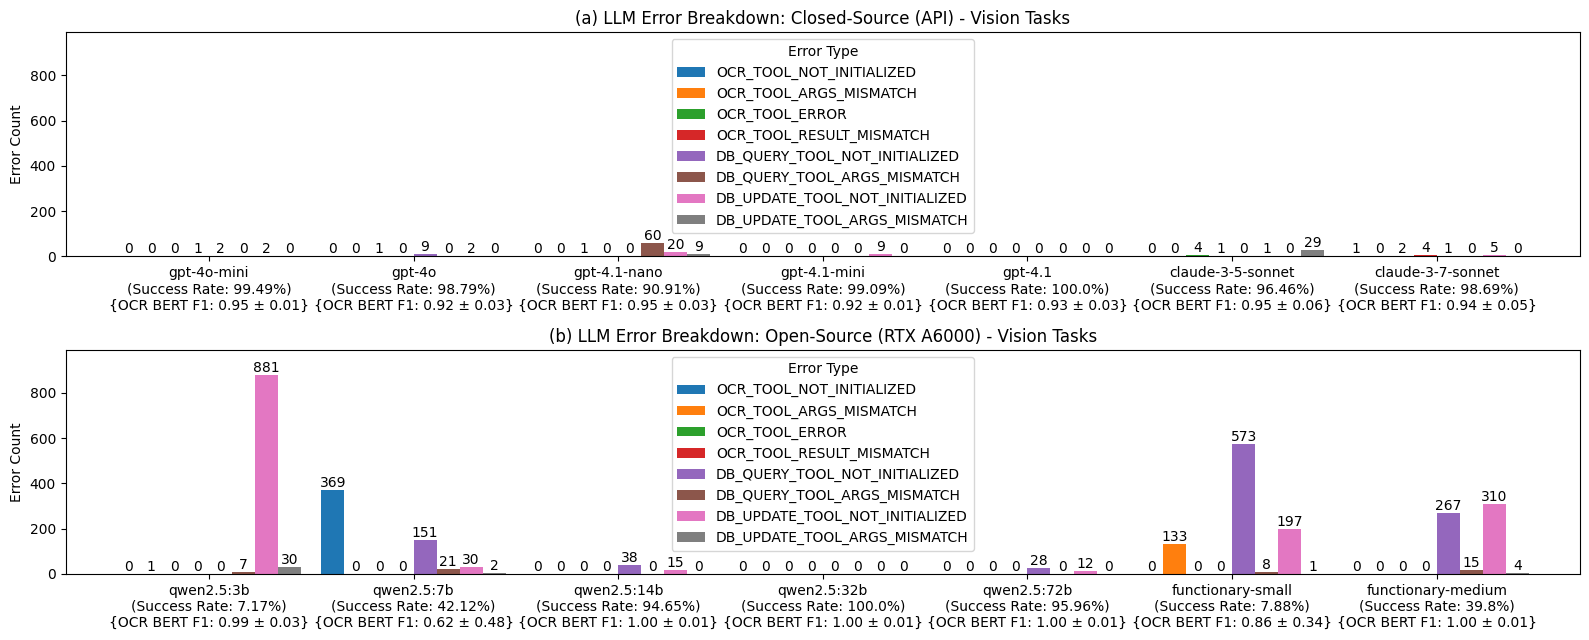
\includegraphics[width=.9\textwidth]{images/error_profiles.png}
    \caption{Systematic error characterization through our diagnostic taxonomy. \textbf{(a)} Closed-source models demonstrate superior procedural reliability with minimal errors. \textbf{(b)} Open-weight models show dramatic variation with scale; initialization failures dominate smaller models. The taxonomy reveals specific targets for system improvement beyond aggregate success metrics.}
    \label{fig:error_profiles}
    \vspace{-1em}
\end{figure*}

\paragraph{Systematic Failure Patterns.}
Tool initialization failures \\(\texttt{DB\_UPDATE\_TOOL\_NOT\_INITIALIZED} and\\ \texttt{DB\_QUERY\_TOOL\_NOT\_INITIALIZED}) dominate error distributions across all model scales. This pattern holds consistently for both vision and non-vision tasks, indicating that procedural invocation—not parameter handling or result interpretation—represents the primary reliability bottleneck. This suggests fundamental challenges in multi-agent orchestration rather than modality-specific limitations.

\paragraph{Model Scale Impact.}
Error rates demonstrate clear inverse correlation with model parameters among open-weight models:

\begin{itemize}
    \item \textbf{Catastrophic failure:} qwen2.5:3b exhibits 881 database update initialization errors (88.99\% of tasks)
    \item \textbf{Moderate improvement:} qwen2.5:14b reduces this to 15--38 errors (1.5--3.8\%)
    \item \textbf{Flawless performance:} qwen2.5:32b achieves zero errors across all categories, matching GPT-4.1
\end{itemize}

This dramatic improvement establishes clear capacity thresholds for production deployment.

% \paragraph{Understanding Initialization Failures.}
% Detailed qualitative analysis of execution logs (Section~\ref{sec:qualitative_analysis}) reveals two distinct reasoning patterns:

% \begin{enumerate}
%     \item \textit{Omission failures:} Models generate conversational responses instead of recognizing tool invocation requirements
%     \item \textit{Malformed call failures:} Models correctly identify tool-use needs but construct invalid function calls with incorrect tool names or malformed JSON structures
% \end{enumerate}

% These findings provide actionable targets for mitigation through improved prompting and system-level orchestration.

% \paragraph{Closed-Source vs. Open-Weight Reliability.}
% Closed-source models demonstrate superior procedural reliability:

% \begin{itemize}
%     \item GPT-4.1 achieves flawless performance (zero errors)
%     \item Even GPT-4.1-nano (85.7\% task success) maintains robust tool-use compared to similarly-sized open-weight alternatives
%     \item This advantage likely stems from extensive instruction-tuning and RLHF specifically targeting tool-use reliability
% \end{itemize}

% \paragraph{Vision Processing Challenges.}
% OCR-related errors exhibit distinct patterns:

% \begin{itemize}
%     \item qwen2.5:7b: 369 initialization failures (37.27\%) with degraded BERT F1 (0.62)
%     \item Functionary-small: 133 argument mismatch errors (13.43\%) despite higher BERT F1 (0.86)
% \end{itemize}

% This divergence suggests OCR accuracy and tool invocation reliability involve separate capabilities requiring independent optimization.

% \paragraph{Diagnostic Insights for System Design.}
% The complete absence of \texttt{DB\_UPDATE\_TOOL\_ERROR} and \texttt{DB\_UPDATE\_TOOL\_RESULT\_MISMATCH} errors in our local SQLite environment suggests these error types would likely emerge in distributed deployments with increased complexity and potential concurrency issues. This highlights important considerations for production system design.

\paragraph{Framework Validation.}
The systematic patterns revealed by our taxonomy demonstrate its diagnostic value. Traditional aggregate success metrics would obscure the critical insight that tool initialization—rather than execution complexity or result interpretation—represents the primary reliability challenge. This granular understanding enables evidence-based decisions about model selection, system architecture, and deployment strategies impossible with coarse-grained evaluation alone.

%%%%%%%%%%%%%%%%%%%%%%%%%%%%%%%%%%%%%%%%%%%%%%%%%%%%%%%%%%%%%%%%%%%%%%%%
\subsection{Qualitative Error Analysis}
\label{sec:qualitative_analysis}
%%%%%%%%%%%%%%%%%%%%%%%%%%%%%%%%%%%%%%%%%%%%%%%%%%%%%%%%%%%%%%%%%%%%%%%%

To complement our quantitative taxonomy, we conducted systematic qualitative analysis of initialization failures—the dominant error type across smaller models. We manually inspected 200 randomly sampled failure cases from execution logs of qwen2.5:3b, qwen2.5:7b, and Functionary-Small to identify underlying reasoning patterns.

% \paragraph{Model-Scale Performance Patterns.}
% Performance patterns reveal that parameter count alone does not guarantee reliability. qwen2.5:7b achieves 737 successful executions (74.3\%), while qwen2.5:3b shows catastrophic degradation with only 68 successes (6.9\%). Notably, Functionary-Small (8B parameters)—despite being larger than qwen2.5:7b—achieves only 132 successes (13.3\%), suggesting that model architecture, training objectives, and instruction-tuning approaches significantly impact multi-agent coordination capabilities beyond raw parameter count. Even the relatively successful 7B Qwen model exhibits recurrent initialization failures, indicating that orchestration-level reliability remains a bottleneck across this parameter range. Models below 14B parameters consistently demonstrate compounded weaknesses including limited context retention, incomplete state propagation, and degraded inter-tool reasoning, with Functionary-Small's particularly poor performance highlighting the importance of training methodology for agentic workflows.

\paragraph{Failure Mode Classification.}
Our qualitative review identifies two dominant failure patterns:

\textbf{Omission Failures ($\approx$68\% of sampled cases).} Agents fail to recognize that tool invocation is required, producing natural-language responses instead. For instance, when prompted to execute a database query, qwen2.5:7b occasionally generates:
    
    \begin{quote}
    \textit{``Based on the invoice information provided, the payment amount is \$1,234.56 for invoice ID INV-2024-001...''}
    \end{quote}
    
    rather than invoking the required \texttt{db\_query\_tool} function. This reflects inadequate procedural reasoning—the model conceptually resolves the task but omits the necessary operational step, revealing weak coupling between semantic understanding and action execution.
    
\textbf{Malformed Call Failures ($\approx$32\% of sampled cases).} Models correctly identify tool-use needs but construct invalid function calls through:
    \begin{itemize}
        \item Incorrect tool names (e.g., \texttt{database\_query} instead of \texttt{db\_query\_tool})
        \item Invalid JSON structure (missing parameters or malformed syntax)
        \item Hallucinated parameters (non-existent fields or incorrect data types)
    \end{itemize}
    These patterns indicate insufficient schema grounding and weak syntactic discipline during tool invocation.

\paragraph{Model-Specific Error Distributions.}
Failure patterns vary systematically across architectures:

\begin{itemize}
    \item \textbf{qwen2.5:3b:} Dominated by omission failures ($\approx$89\% of sampled errors), reflecting shallow procedural reasoning and weak context maintenance
    
    \item \textbf{qwen2.5:7b:} Predominantly omission failures with high argument precision when tools are invoked%; most errors represent isolated initialization lapses
    
    \item \textbf{Functionary-Small:} 
    Balanced distribution ($\approx$55\% omission, 45\% malformed)
\end{itemize}

% \paragraph{Design Implications for Robust Systems.}
% Our findings motivate several architectural interventions:

% \begin{enumerate}
%     \item \textbf{Dedicated Orchestration Layer:} Implement explicit controllers for tool initialization, validation, and dependency tracking to reduce errors through systematic state management
    
%     \item \textbf{Schema-Aware Tool Invocation:} Employ structured decoding or JSON schema validation to enforce syntactic correctness
    
%     \item \textbf{Persistent Context Management:} Maintain shared state across invocations through external memory, particularly critical for models with limited context windows
    
%     \item \textbf{Adaptive Error Recovery:} Deploy dynamic retry strategies with graceful degradation, enabling recovery from transient failures
    
%     \item \textbf{Reinforced Procedural Prompting:} Mitigate omission failures through explicit tool-use signals or fine-tuning with execution feedback
% \end{enumerate}

Overall, our qualitative analysis reveals that tool-calling failures in smaller models stem from two main issues: failure to initiate tool use and incorrect execution of tool calls. While larger models like qwen2.5:7b show improved precision, they still suffer from procedural lapses such as omission errors. Reliable multi-agent systems will require not just capable models but also robust orchestration mechanisms, schema-aware invocation, and strategies for error recovery to mitigate these recurring failure modes.

% %%%%%%%%%%%%%%%%%%%%%%%%%%%%%%%%%%%%%%%%%%%%%%%%%%%%%%%%%%%%%%%%%%%%%%%%
% \subsection{Edge Deployment Feasibility and Practical Guidance}
% %%%%%%%%%%%%%%%%%%%%%%%%%%%%%%%%%%%%%%%%%%%%%%%%%%%%%%%%%%%%%%%%%%%%%%%%

% Our hardware characterization and error analysis converge on practical deployment guidelines for resource-constrained environments. The 14B parameter threshold emerges as critical for reliable multi-agent coordination on commodity hardware, balancing task success rates (96.6\%) with acceptable latency (7.3--12.5~seconds on RTX 4090/A6000). Larger models provide diminishing returns for this task complexity, while smaller models require substantial architectural compensation.

% For deployments below the 14B reliability threshold, validation layer design guided by our diagnostic taxonomy becomes essential. Organizations can achieve acceptable failure rates through systematic error detection, automated retry mechanisms, and human-in-the-loop escalation for high-confidence failures. This tiered approach enables SMEs to deploy multi-agent systems aligned with their specific cost-reliability trade-off preferences.

\section{Conclusion}
\label{sec:Conclusion}

This work introduces a systematic diagnostic infrastructure for evaluating tool-use reliability in multi-agent LLM systems, addressing a critical gap in existing evaluation frameworks. Our 12-category error taxonomy enables fine-grained characterization of procedural failures, revealing actionable insights often obscured by aggregate success metrics.

An analysis of 1,980 deterministic test instances yields three key findings:  
(1) Tool initialization failures—rather than parameter tuning or output interpretation—emerge as the primary reliability bottleneck. These failures occur at catastrophic rates in small models (e.g., qwen2.5:3b: 89\% errors) and are entirely absent in large models (e.g., qwen2.5:32b, GPT-4.1: 0\% errors);  
(2) Distinct capacity thresholds are observed at 14B parameters (minimum viable, with 96.6--97.4\% success) and 32B parameters (achieving reliability parity with closed-source models);  
(3) Hardware exerts a substantial influence, with up to 8.2$\times$ latency variation across platforms and failure modes such as recursive loops and forced terminations on underpowered systems.

% A qualitative review of 200 sampled failures reveals two dominant error categories: omission errors (68\%), where models respond conversationally instead of invoking tools; and malformed calls (32\%), such as invalid tool names, malformed JSON, or hallucinated parameters. Error patterns vary across models, highlighting actionable targets for orchestration layers, schema validation, and prompt design reinforcement.

Based on our findings, we propose tiered deployment recommendations to balance reliability and cost:  
qwen2.5:32b on RTX A6000 (\$10K) delivers flawless performance, matching GPT-4.1;  
qwen2.5:14b on RTX 4090 (\$5K) offers strong accuracy-efficiency trade-offs suitable for most applications;  
Sub--14B models require substantial architectural augmentation—including validation layers, retry logic, and human oversight—to achieve acceptable reliability.

Future directions include:  
(1) adversarial and negative-case protocol design;  
(2) distributed failure analysis; 
% CHANGE: Added future work discussion on self-healing mechanisms as suggested by reviewer
% Rationale: Reviewer suggested discussing how error categories could inform "self-healing" or corrective mechanisms
(3) self-healing agent architectures informed by our taxonomy, where error category detection triggers automated corrective mechanisms such as prompt reformulation for omission failures or schema validation for malformed calls; and  
(4) cross-domain validation beyond finance.

As multi-agent LLM systems move from prototypes to production, ad hoc evaluation no longer suffices. Our diagnostic framework shifts evaluation from whether a system works to why it fails, providing a reproducible, fine-grained method for measuring procedural reliability and enabling more robust, predictable, and trustworthy agentic AI for real-world deployment.

% As multi-agent LLM systems progress from academic prototypes to production-grade deployments, ad hoc evaluation methods are no longer sufficient. Our diagnostic framework represents a necessary evolution—shifting focus from whether a system works to why it fails. By providing a reproducible, fine-grained methodology for evaluating procedural reliability, this work lays the foundation for building more robust, predictable, and trustworthy agentic AI. It marks a critical step toward the engineering maturity required for deploying complex AI systems safely and effectively in real-world settings.


%%%%%%%%%%%%%%%%%%%%%%%%%%%%%%%%%%%%%%%%%%%%%%%%%%%%%%%%%%%%%%%%%%%%%%%%

\bibliographystyle{IEEEtran}
\bibliography{references}

\end{document}